\section{Design af Controller}

Det endelige mål med kontrolsystemet er at kunne styre orienteringen af rammerne præcist ved at give et vinkel-input. Dette input konverteres så til et fejlsignal som er forskellen imellem den ønskede vinkel og den faktiske vinkel som systemet står i. Controllerens opgave er så, at holde øje med fejlen og derigennem beregne sig til en passende PWM duty cycle, så input og output til sidst stemmer overens. 

\begin{figure}[ht]
	\begin{center}
		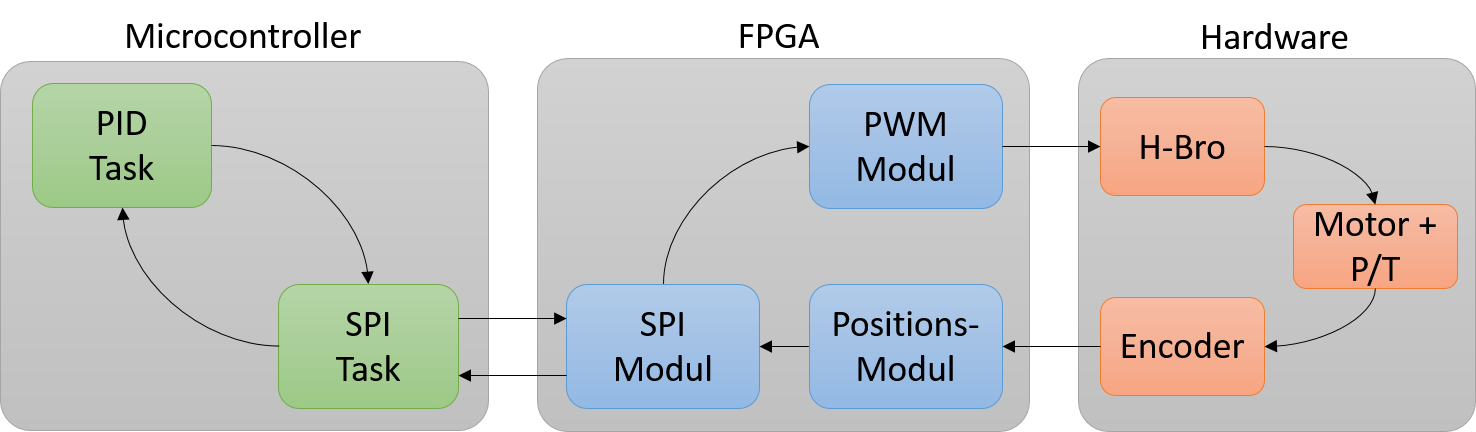
\includegraphics[scale=0.5]{Billeder/Controller_Blok.png}
	\end{center}
\caption{Her ses data flowet for kontrolløkken.}
\label{fig:Blok_Model}
\end{figure}

På figur \ref{fig:Blok_Model} kan man se de vigtigste elementer i kontrolløkken fra microcontrolleren og ud til selve systemet. Ud fra et modelleringsperspektiv er de fire mest interessante dele af systemet som følger:

\begin{itemize}
\item \textbf{H-bro}: Sørger for at regulere forsyningsspændingen på 12V til motoren alt afhængig af den duty cycle som PWM-modulet sender ud. Duty cycle styrer den gennemsnitlige spænding over motorterminalerne. H-broen kan også vende strømmen igennem motoren for at skifte omdrejningsretningen.
\item \textbf{Motor og Pan/Tilt-system}: Producerer en omdrejningshastighed, som er relateret til spændingen over motorterminalerne ved overføringsfunktionen beskrevet i ligning (\ref{eq:tf_pan_tilt}).
\item \textbf{Encoder og Positionsmodul}: To hall sensorer i encoderen genererer pulser, der gør det muligt at bestemme omdrejningsretningen for motoren. Positionsmodulet sørger for at holde styr på pulserne, for at afkode hvilken stilling motoren har stillet sig i. Dette er muligt hvis man starter med at have en fast reference man tæller fra.
\item \textbf{Controller}: Sørger for at generere et passende PWM-signal, så motoren kan flytte rammerne over i den ønskede position. Dette skal foregå på en måde, så designmålene for projektet overholdes.
\end{itemize}

Modelleringen af systemet viste at motoren og pan/tilt-systemet kunne approksimeres nogenlunde som et 1.-ordenssystem.
Hvis man tager udgangspunkt i grey box-modellen af systemet, kan man lave et closed-loop-system, der ser ud som på figur \ref{fig:BB_Model}. På denne model er H-broen modelleret som et gain på 12. PWM-signalet kan variere fra $-1$ til $1$. Encoderen og positionsmodulet fungerer i praksis lidt som en integrator i den forstand at alle ticks summeres op og giver en relativ position. Der er ikke noget gain igennem feedback-løkken da set point'et til controlleren også opgives i ticks. Det vides på forhånd at et tick svarer til $1/3$ af en grad (XXXX se reference her), så for at holde kontrolsystemet simpelt, foretages den omregning inden set point'et gives til controlleren.

\begin{figure}[ht]
	\begin{center}
		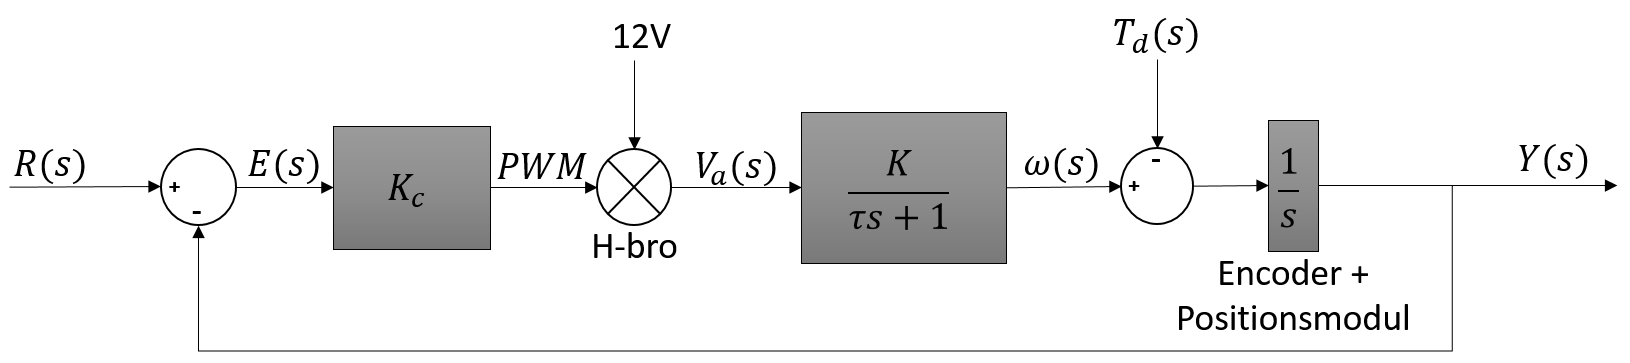
\includegraphics[scale=0.5]{Billeder/Control_Loop.PNG}
	\end{center}
\caption{Closed-Loop kontrolsystem til grey box-modellen}
\label{fig:BB_Model}
\end{figure}

\subsection{Designmål}

\begin{itemize}

\item Steady state fejl på 0
\item Overshoot $<$ 15 $\%$
\item Settling time $<$ 5 sekunder

\end{itemize}

\subsection{2.-ordenssystem}

Når man designer en controller, kan det være praktisk at approksimere hele systemet som et ideelt 2-ordens-system (se ligning \ref{eq:SO_system}). Disse systemer er meget veldefinerede og forholdsvis lette at beregne på. Parametre som overshoot, settling time, rise time m.m. kan beregnes analytisk og kan give et godt udgangspunkt til ens valg af controller. $\omega_{n}$ er systemets naturlige frekvens og $\zeta$ er systemets damping ratio - jo større en damping ratio, jo bedre en dæmpning af systemets respons har man.

\begin{equation}\label{eq:SO_system}
Y(s)=\frac{\omega_{n}^2}{s^2+2\zeta\omega_{n}s+\omega_{n}^2}
\end{equation}

Hele ideen med at benytte et 2-ordens-system til den indledende analyse, er at man kan finde de områder i s-planet, hvor systemet vil holde sig inden for designmålene, så længe systemets poler placeres der. Disse antagelser gælder naturligvis kun præcist for et 2-ordens-system uden nuller, men det kan sagtens være en udemærket approksimering, hvis man har et system af højere orden med to dominante poler der ligger tæt på $j\omega$-aksen. Som tommelfinger-regel kan man godt tillade sig at kalde to poler for dominante, hvis de er 5 gange tættere på den imaginære akse end resten af polerne. Grunden til at man kigger mest på de dominante poler, er at jo længere man kommer væk fra $j\omega$-aksen jo hurtigere aftager effekten på systemet fra polerne over tid. Derfor ender det med at være de langsomme poler, der dominerer systemets respons.



På figur \ref{fig:SO_system} kan man se hvordan man alene ud fra polernes placering kan beskrive en masse om damping ratio og den naturlige frekvens. En ting der ikke fremgår af figuren, er at damping ratio også fortæller noget om, om polerne er komplekse konjugerede eller reelle. Hvis $1>\zeta>0$ er polerne komplekse; hvis $\zeta=1$ ligger der to reelle poler oven i hinanden; hvis $\zeta>1$ er polerne reelle og unikke. Disse tre situationer bliver også ofte beskrevet som henholdsvis underdæmpet, kritisk dæmpet og overdæmpet.

\begin{wrapfigure}[15]{l}{0.5\textwidth}
\vspace{-20pt}	
	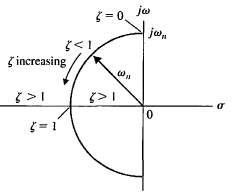
\includegraphics[scale=0.5]{Billeder/Damping_Ratio.PNG}
	\centering
	\vspace{-10pt}
	\caption{Her kan man se hvordan damping ratio og den naturlige frekvens påvirker polernes placering i et 2-ordens-system.}
	\label{fig:SO_system}
\vspace{-20pt}
\end{wrapfigure}


\subsubsection{Steady State Fejl}

For at undersøge om systemet kan drive fejlen i 0, er det nødvendigt at finde et udtryk for $E(s)$, som kan ses på figur \ref{fig:BB_Model}, og ved hjælp af \textit{Final Value Theorem} (ligning \ref{eq:FVT}), finde ud af hvad der er tilbage, når systemet går i steady state. 

\begin{equation} \label{eq:FVT}
lim_{t \to \infty} f(t) = lim_{s \to 0} sF(s)
\end{equation}

\begin{equation} \label{eq:ess}
E(s)=R(s)\frac{s(\tau s+1)}{s(\tau s+1)+12K_{c}KH}+T_{d}(s)\frac{(\tau s+1)H}{s(\tau s+1)+12K_{c}KH}
\end{equation}

Ved et step-input ($A/s$) bliver fejlen drevet i 0, så længe der ikke er nogen disturbance. 

\begin{equation}
e_{ss}=lim_{s \to 0} sE(s)=AH\frac{1}{12K_{c}KH} , T_{d}(s)=\dfrac{A}{s}
\end{equation}

Det kan altså konkluderes, at man er nødt til at have mindst en integrator i controlleren ($K_{c}$), for at opfylde kriteriet om en steady state-fejl på 0. 

\subsubsection{Overshoot}

Percent Overshoot (P.O.) er defineret som den procentdel systemets største respons afviger fra den ønskede værdi - det er et udtryk for, hvor meget systemet skyder forbi målet når det påvirkes af et step input. Ved hjælp af lidt algebra, differentiering og et par laplace-transformeringer, kan man udlede ligning (\ref{eq:P.O.}) fra ligning (\ref{eq:SO_system}) (se Modern Control Systems\cite{ModernControlSystem}), og på den måde finde ud af, hvor meget overshoot systemet har udelukkende ud fra damping ratio. En anden måde at se på problemet, er at man, ved at finde zeta til et bestemt overshoot, også kan finde den vinkel til de komplekse polers placering, hvor man får netop den mængde overshoot - store vinkler giver stort overshoot og omvendt (se figur \ref{fig:SO_system}). Man kan altså ud fra denne udregning definere et klart område, hvor alle polplaceringer vil opfylde ens krav til overshoot. 

\begin{equation}\label{eq:P.O.}
P.O.=100*e^{-\dfrac{\zeta\pi}{\sqrt{1-\zeta^2}}}
\end{equation}

For at få 15 $\%$ overshoot eller derunder kan det beregnes at $\zeta$ skal være større end 0.517. Det vil sige at polerne skal placeres indenfor det skraverede område på figur \ref{fig:Overshoot} for at opfylde designmålene. Det er værd at nævne igen, at dette kun viser opførslen for et 2-ordens-system, så man kan ikke præcist beskrive opførslen for vores system på denne måde. Til gengæld kan man, hvis man tænker sig om under controller-designet, komme meget tæt på. Det er dog stadigvæk smart at vælge polplaceringer med en god margen op til grænseværdien for at være på den sikre side.

\begin{figure}[ht]
	\begin{center}
		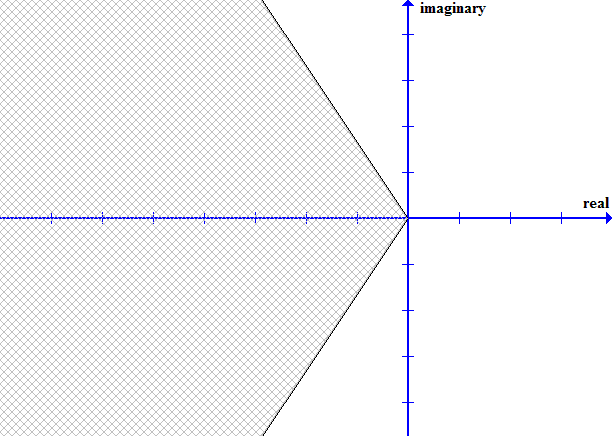
\includegraphics[scale=0.5]{Billeder/Overshoot.PNG}
	\end{center}
\caption{Det skraverede område viser alle punkter med en zeta-værdi over 0.517. Denne værdi svarer også til en vinkel til den reelle akse på 58.87 grader til begge sider}
\label{fig:Overshoot}
\end{figure}

\subsubsection{Settling Time}

Settling time er defineret som den tid det tager systemet at falde til ro inden for 2 procent af den ønskede værdi. Hvis man kigger på formlen for impulsresponsen (ligning (\ref{eq:impulse_response}))  til et 2-ordens-system i tidsdomænet, kan det ses at den dæmpende faktor for systemet er $e^{-\zeta\omega_{n}t}$ - settling time så beskrives ved $e^{-\zeta\omega_{n}T_{s}}<0.02$ og herfra kan man udlede ligning (\ref{eq:settling_time}).

\begin{equation}\label{eq:impulse_response}
y(t)=\frac{\omega_{n}}{\beta}e^{-\zeta\omega_{n}t}Sin(\omega_{n}\beta t)
\end{equation}

\begin{equation}\label{eq:settling_time}
T_{s}=\frac{4}{\omega_{n}\zeta}
\end{equation}

For at få en settling time på under $5s$ kan det ud fra ligning (\ref{eq:settling_time}) bestemmes at $\omega_{n}\zeta > 0.8$. Det vil med andre ord sige at polerne skal befinde sig til venstre for -0.8 - her refereres der igen til figur \ref{fig:SO_system}. Ligesom det var tilfældet for overshoot-kriterierne, er det også her en god ide at vælge sine poler med en god margen til grænseværdien.

\paragraph{Delkonklusion}

For at overholde designmålene vedrørende settling time, overshoot og steady state fejl, kan det følgende konkluderes:

\begin{itemize}
\item Damping ratio for et 2.-ordenssystem skal være større end $0.517$.
\item Produktet $\omega_{n}\zeta$ for et 2.-ordenssystem skal være større end $0.8$. Dette produkt svarer til den reelle komponent af to komplekse poler.
\item For at holde steady state fejlen i 0, skal man have en controller med et integrator led. Derfor skal det undersøges hvordan en I-, en PI- og en PID-controller påvirker systemet. P- og PD-controllere ignoreres pga af kravet til steady state fejlen.
\end{itemize}

Grænserne skal ses som et absolut minimumskrav, da systemet ikke er et ideelt 2.ordenssystem. Der skal helst være en god margen.

\subsection{I Controller}

En I-controller er et integrator-led med et gain - integratoren svarer til at placere endnu en pol i origo. For at undersøge hvordan denne controller vil opføre sig, kan man bruge root locus metoden for at se, hvordan polerne flytter sig, når controller-gainet øges. 

\begin{equation}\label{eq:I_OpenLoop}
Y(s)=K_{I}\cdot\frac{1}{s}\cdot\frac{12K}{s(s\tau+1)}
\end{equation}

For at plotte root locus i matlab skal man bare bruge open loop overføringsfunktionen (ligning \ref{eq:I_OpenLoop}). På figur \ref{fig:I_rlocus} ses det med al tydelighed at systemet aldrig bliver stabilt med en I-controller, da polerne ikke kan trækkes over på den negative side af $j\omega$-aksen. Af denne grund kan en ren I-controller ikke bruges.

\begin{figure}[ht]
	\begin{center}
		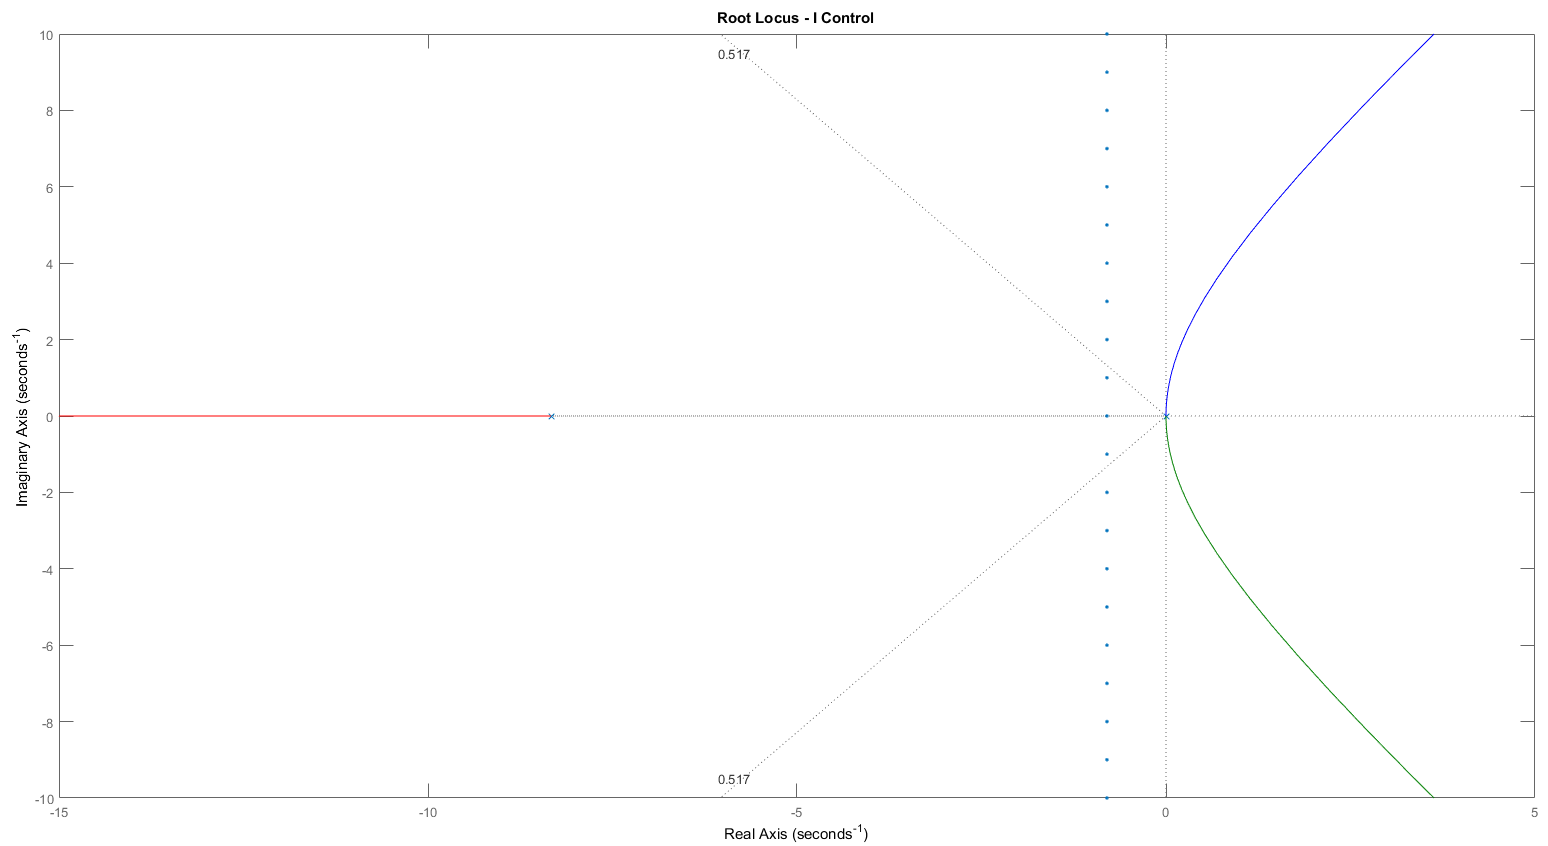
\includegraphics[scale=0.35]{Billeder/I_rlocus.PNG}
	\end{center}
\caption{Her ses root locus plottet for vores system med en I-controller. Det er tydeligt at systemet aldrig kan stabiliseres med et gain alene. Dette plot er lavet med en tidskonstant på 0.12 sekunder, hvilket vil svare til en pol i -8.33.}
\label{fig:I_rlocus}
\end{figure}

\subsection{PI Controller}

En PI controller har også en proportionel del, der summeres med integratoren. Det resulterer i praksis i at der, udover polen i origo fra integratoren, også tilføjes et nul på ventstre side af den imaginære akse. Nullets placering bestemmes af forholdet imellem $K_{I}$ og $K_{P}$.

\begin{equation}\label{PI_OpenLoop}
Y(s)=\frac{K_{P}s+K_{I}}{s}\cdot\frac{12K}{s(s\tau+1)}
\end{equation}

Ud fra root locus beregninger kan det bevises at nullets placering skal ligge til højre for $-0.93$ for at de to branches fra polerne i origo mødes på den reelle akse. (XXXX Skal beviset udpensles med ligninger eller er det fint bare at sige det passer?). $K_{P}$ skal med andre ord helst være større end $K_{I}$. Til gengæld må $K_{P}$ heller ikke blive for meget større end $K_{I}$ (knap $2.6$ gange) fordi det gør systemet for langsomt, da break-in punktet kommer til at ligge på den forkerte side af $0.8$, som er $\omega_{n}\zeta$-grænsen for en settling time under 5 sekunder. 

\begin{equation}
1+G\frac{(s+I/P)K}{s^2(\tau s+1)}=0
\end{equation}

\begin{equation}
G=-\frac{s^2(\tau s+1)}{(s+I/P)K}
\end{equation}

\begin{equation}
\frac{dG}{ds}=0
\end{equation}

\subsection{PID Controller}

\begin{equation}\label{PID_OpenLoop}
Y(s)=\frac{K_{P}s+K_{I}+K_{D}s^2}{s}\cdot\frac{12K}{s(s\tau+1)}
\end{equation}

Med PI-controlleren er margenen for P- og I-konstanterne og gainet ret snæver, hvis projektets designmål skal overholdes. PID-controlleren giver lidt mere råderum, men man tager også et skridt længere væk fra den ideelle 2.-ordensmodel. Differentieringsledet D tilføjer nemlig et ekstra nul til ligningen. Med to nuller er der ikke længere to branches, der går mod uendelig langs en lodret asymptote når gainet øges. Der er nu kun en branch der går mod minus uendelig, og det foregår langs den reelle akse. Dette har tre klare fordele:

\begin{itemize}
	\item 	En af polerne fra det modellerede 3-ordens-system glider væk fra de to andre poler ved højere gain. På den måde kan man lettere negligere effekten fra den i modellen.
	\item  	Man kan altid sørge for at de to dominante poler befinder sig på den 				   	reelle akse (mindre overshoot), hvis de to tilføjede nuller også er reelle og gainet er tilpas stort. 
	\item  	Man kan få de to dominante poler længere væk fra den imaginære akse 					(hurtigere settling time).
\end{itemize}

I de root locus-plots der har være vist indtil videre, har der været brugt en tidskonstant på 0.12 sekunder - denne værdi stammer fra forsøg på tilt-systemet. Med denne tidskonstant får man en pol på $-1/0.12=-8.33$. Hvis begge nuller placeres til højre for $-8.33$ vil den ene branch følge den reelle akse til venstre for $-8.33$ mod uendelig. På den måde kan man, med et forholdsvist lille gain, skubbe closed-loop-polen fra tidskonstanten så langt ud ad den reelle akse, at den ikke har nogen stor indflydelse på systemet. Det kan også lade sig gøre, hvis et af nullerne eller begge to er til venstre for $-8.33$, det kræver bare et noget større gain.

\begin{figure}[ht]
	\begin{center}
		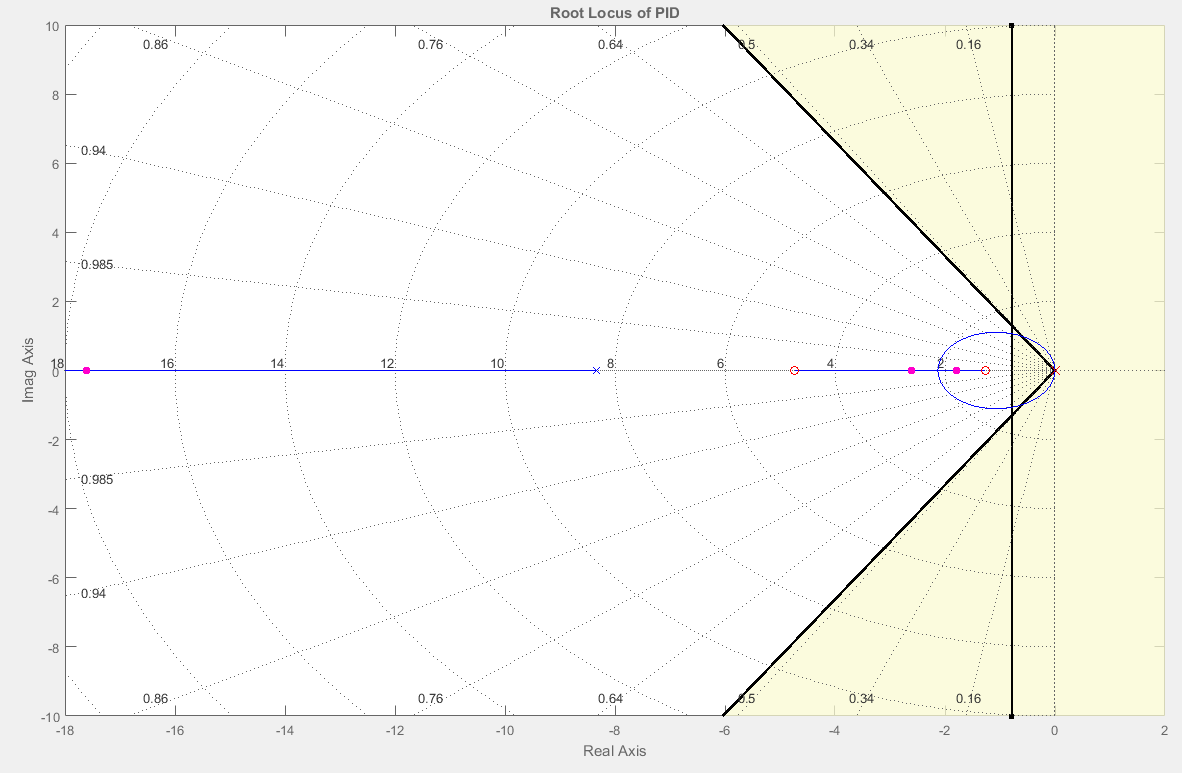
\includegraphics[scale=0.45]{Billeder/PID_rlocus.PNG}
	\end{center}
\caption{Her ses root locus plottet for vores tilt-system med en PID-controller med P=6, I=6, D=1 og et gain på 0.0027}
\label{fig:PID_rlocus}
\end{figure}